\chapter{Test}
In this chapter, we go through the tests, which got made during the development of the Ezuino programming language. At the beginning of the project, the only tests which could be done were using the language made by the ANTLR grammar file and testing different dummy programs, and test whenever ANLTR report any ambiguity or syntax error within the code entered. Multiple programs got written, to ensure that we got around every syntax and scenario possible, to avoid any future error, once we’ve started building the Concrete Syntax Tree (CST) and the Abstract Syntax Tree (AST).  One of the programs can be reviewed in figure \ref{test0} and \ref{test00}.

\begin{figure}[H]
\centering
\frame{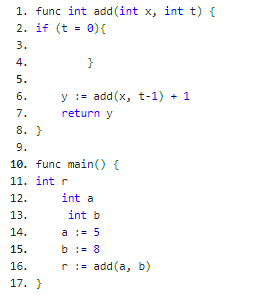
\includegraphics[scale=1]{figures/test/test0.png}}
\caption{Test}
\label{test00}
\end{figure}

\begin{figure}[H]
\centering
\frame{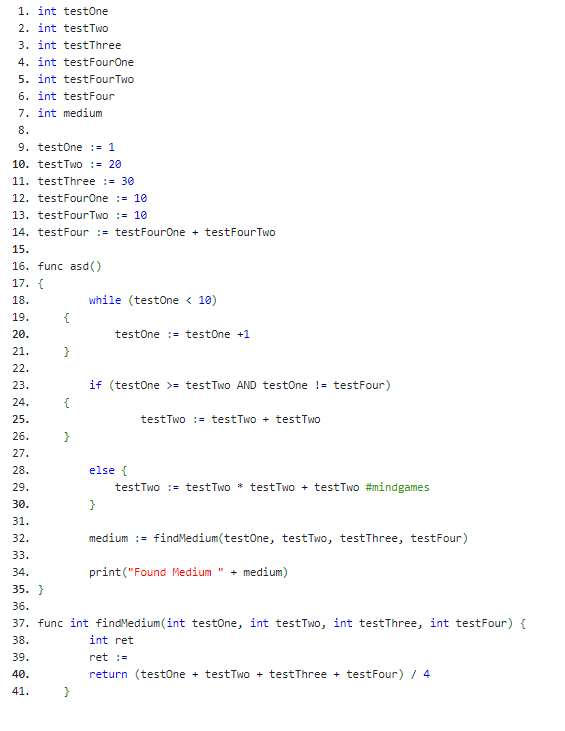
\includegraphics[scale=1]{figures/test/test6.png}}
\caption{Test}
\label{test0}
\end{figure}

\section{JUnit Testing}
Once the development of the compiler in Java has started, JUnit testing has been used during the remaining of the process. This section will go through some of the JUnit test, which gets written during the development process. The tests have been categorized into three sections: CST, AST, and Lexer/Parser test. 
Starting from the beginning of development, we get to look at the Lexer/Parser test, which is the classes ANTLR 4 has generated and using the ANTLR maven package, can use. In these test classes, we use the Error Handler, which was explained the chapter 6, to check whenever there is an error, during the lexing/parsing of a small code snippet. If the error handler finds an error, depending on the asset, the test will either fail or pass. 
\begin{figure}[H]
\centering
\frame{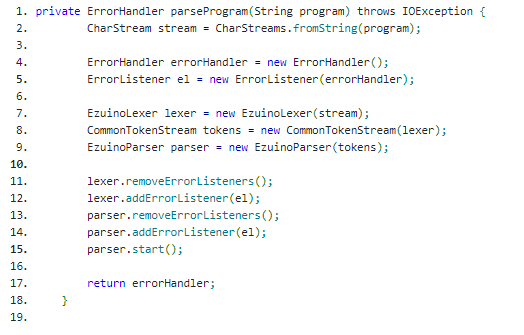
\includegraphics[scale=1]{figures/test/test2.png}}
\caption{Test}
\label{test1}
\end{figure}
Figure \ref{test1} shows a method, which is used to initialize the error handler, lexer and parser with the code, as inputted by a string. 
\begin{figure}[H]
\centering
\frame{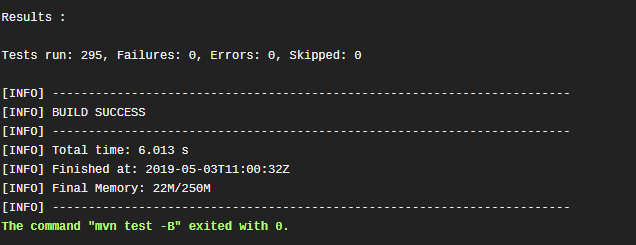
\includegraphics[scale=1]{figures/test/test4.png}}
\caption{Test}
\label{test2}
\end{figure}
On figure \ref{test2}, we have the first test, which a simple integer declaration, where we declare the variable a. We assert that the errorhandler should’t have any errors, as this is the correct syntax in this case – using the hasErrors() method, which is a part of the error handler class, and will return an Boolean value. 
Moving on towards the type checker and CST tests, test on figure 4 shows a test with a multiplicative expression: 
\begin{figure}[H]
\centering
\frame{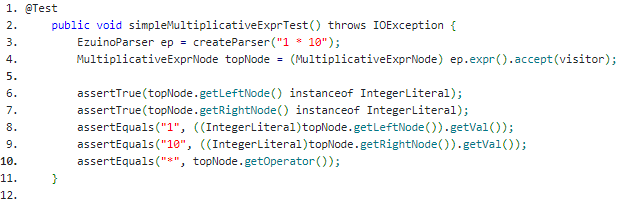
\includegraphics[scale=0.86]{figures/test/test5.png}}
\caption{Test}
\label{test3}
\end{figure}
Figure \ref{test3} shows the test of the expression (1 * 10), where we test if both the right and left side nodes of the MultiplicativeExprNode is of type Integers. If they aren’t, we can already throw an exception. Next, we’re checking if the values of the left and right node are the ones which we’ve entered in our expression. In this case, we assert that the left node has the value 1, and the right node has the value 10.  We also check that the operator in this expression is a multiplicative operator.
The code generation tests for Java bytecode and C, has been tested by taking the Ezuino program, and comparing it to an expected output of the C programming language. If the output is correct, the tests are successful.  
\section{Continuous Integration}
During the development of the programming language, more tests has been added in the development process. The final number of tests, is around 250+, in multiple classes. This is a significant number of tests to run each time an AST or node has been changed, so Continuous Integration (CI), has been deployed, to automate each test and compile the software after each Git Commit (GC) or Pull Request (PR).  The CI used for this purpose was Travis CI, which is a free CI service for public git repositories. \\
\begin{figure}[H]
\centering
\frame{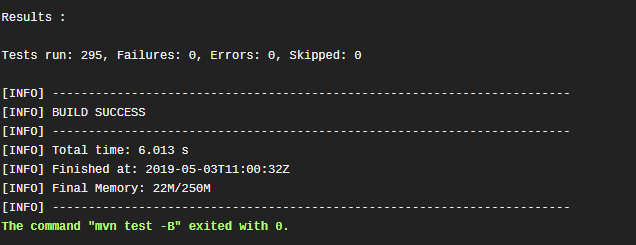
\includegraphics[scale=0.8]{figures/test/test1.png}}
\caption{Test}
\label{testa}
\end{figure}
On figure \ref{testa}, a Travis build has run on a GC, which has recently been committed. In this result, we can see that the 295 tests have been ran successfully, and the program ran without any error. In case the program finds an issue, and add it to the Error Handler, it will fail the build, but no the tests. Also, the other way around, if a node has been changed, but the program may build, if one tests fails, the Travis check will fail as well. \\
\\
This chapter has been going through a few of the around 300 tests made in this project, and given an insight in the tests process which has been made during the development of the Ezuino programming language. It is very essential to avoid errors in the compiler in a programming language, so testing of features has been prioritized, however, there are still testing forms like code coverage and whitebox (branch testing), which has not been done at this time. If the Ezuino programming language were to get a commercial release, these tests are essential to provide a large sum of error or failure correction, as a programming language is very abstract. 
\section{User Test}
In this chapter we present the feedback we were given from on Ezuino. The test person was a student in psychology second semester having never programmed before but interested in participating in the test. The test was conducted by giving the test person a guide that both covered basic programming terms, the syntax of Ezuino with code examples and a set of assignments. The guide can be seen in appendix \ref{user_guide_appendix}. The test person was taking the test together with a test moderator, in order to ensure the participant did not get completely stuck at an task either due to being completely new to programming or due to the guide being unclear. After the test the participant was asked give feedback on the programming language and to review key points about Ezuino where it differed from C. The screen and communication during the test was recorded for intern review with consent.
We got the following feedback
\begin{itemize}
    \item "AND" and "OR" was preferable to  $\&\&$ and $\|\|$ and boolean was prefered to 0 and 1. 
    \item The data types could be less technical named so it is easier to understand without a background. An example from the test person was that string could be called "words". We asked if "text" would also be easy to understand as we felt it was more precise for more use cases of strings, and the test person said it was just as good. It could be observed from the test person that they fairly fast forgot was the meaning of int, double and boolean was after having read the explanation. While this could simple be due to having to comprehend many programming terms in a short time span, it could also be due to the name of the data types being less intuitive, making them harder to remember the meaning of.
    \item Strong typing also came as a surprise to the test person. That 32 gave an type error when assigned to double was an example of this.
    \item We showed the test person the list we had intended to implement as versions of arrays that did not need malloc and free and functioned like ArrayList in Java but without being object oriented. The test person did prefer it, but also suggested a method to find the index of a value in a string list in case they had a hard time keeping track of what index each value was saved. Interestingly enough the index of an value is often easier to remember in arrays compared to list when looking at source code, since you have use the array index when you assign entries in an array. This suggest that having both arrays and a structure similar to list would be good since they both have different advantages for people new to programming. In both arrays and list the test person would prefer that entries in the array would start from index 1 instead of 0.
    %\item To our surprise the test person did not dislike the idea of ending statements with ";" like in C, comparing it to dot in a sentence. According to the test person dot could even substitute ";". In the same manner of thought the test person also suggested that the starting letter of keywords that can start a line could also start with uppercase, making it more like an sentence.
    \item According to the test person ":=" and "=" made sense compared to C, ":=" reminding the test person of assignment in a math program previously used in her study.
    \item During the test there were a few times the test person forgot declaration before assignment. This could be interpreted as declaration before usage being unintuitive to new programmers. 
\end{itemize}

Besides those points the test person also gave some feedback on our current error messages, making us aware that both the error messages from type mismatch and syntax error had some room for improvement.









%This guide can be seen in appendix (SKRIV APPENDIX IND).  
%The test setup is simple. A table, with a chair together with a computer running a text editor with one text file “code.ezuino”, and running the programming language in the background. After the compiler has compiled the program, the output program was then copied into an Arduino IDE, and executed on the Arduino. The test person was handed a syntax specification table, which contain a small explanation of what each operator did, and we tried to give them two simple tasks, which they will use the language, only using the syntax specification table. \\
%\\
%The first test which got presented to the test person were a simple programming task, where they had to construct a “hello world” string in a function, which is outside the setup and loop function, and run it the function once. At first, the test person was confused, however, after presenting them to how the setup and loop functions works, and told them what each of them did, they replicated a function, similar to the setup function, and insert a print statement, which printed “hello world”. The test person had an issue understanding functions, as they wanted to run the program right after they have added their new function. When a dialog with the test person, on how functions work, and that the code only executes the setup and main, and you must call the function in each, the test person completed this task.\\
%\\
%The second test which got presented to the test person, were harder task, but builds on the previous task, and provides a code example written C, with Arduino libraries attached. The tasks were to learn about the user’s interaction between the Arduino and applying code to get a result. The programming was to get data from a temperature sensor and get the temperature out in the Arduino console. By already providing the body, with setup, loop and serial begin as the first test setup, the only explanation we gave the test person beforehand, was that floats form the program example was double in our language, and that they had the same functionality. As the Ezuino programming language already had a lot of the library features which Arduino reside, the user could replicate the code into the Ezuino programming language, with one missing component, the language was missing (println – prints on a new line). We asked the test person whenever he understood the difference between the normal print and the print new line method, and he answered yes, and concluded that it could be a good feature to include.\\
%\\
%We can conclude from this limited test that language specification and documentation are everything. Good explanations of where to start, what each do, and where to use each feature where is vital, and can get people, with no programming experience to produce functional code. In goal with this project, is to avoid having a teacher, sitting next to the person programming, but to learn it from a set of instruction and specification. The test setup with the temperature sensor used for the second test was not user friendly for users who do not have experience at all. If home automation for Arduino would ship, we should provide easy and ready packages, where the user only should plug the Arduino into their computer and execute the code. At last, there was a feature which we did not think should have been added. The println feature was understood by the user, and as it can provide a good functionality to the program, we added this feature in the language.
%\\